\documentclass[UTF-8]{ctexbeamer}
\usetheme{Boadilla}

\usepackage{listings}

\title{MeowV64}
\subtitle{对于并行执行的一些尝试}

\author{Grp.3 - 刘晓义\hspace{.2em} 娄晨耀 \hspace{.2em} 郑林楷 \hspace{.2em} 申奥}
\date{2019.12.27}

\begin{document}
\begin{frame}
  \titlepage
\end{frame}
\begin{frame}
  \frametitle{Repository \& Contribution}

  \textbf{https://github.com/meow-chip/MeowV64}

  \vspace{1em}

  \begin{description}
    \item[刘晓义] 其他的一些东西(?)
    \item[娄晨耀] BPU, Cache
    \item[申奥] BPU, ALU
  \end{description}
\end{frame}
\begin{frame}
  \frametitle{Features}

  \begin{itemize}
    \item RISC-V, RV64IMAC -Zifencei -Zicsr
    \item 双周期处理器
    \pause
    \item 流水线支持 Superscalar 乱序执行 \& 预测执行
    \item L1/2 Cache 支持多核一致性协议
    \item 可配置:发射数,Cache 大小、组相联,Inflight instr count, \textbf{执行单元}
  \end{itemize}
\end{frame}

\begin{frame}
  \frametitle{Fetch}

  \begin{columns}
    \column{0.3\textwidth}
    \begin{itemize}
      \item 支持变长指令:相邻指令会重叠
      \item 支持多发射:BHT 同一行存储多个结果
      \item ?-bit BHT
      \item Flush
      \item FENCE.I
      \item TODO: RAS?
    \end{itemize}
    \column{0.7\textwidth}
    \begin{center}
      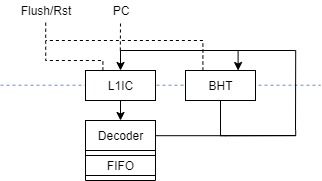
\includegraphics[width=0.8\textwidth]{assets/fetch.jpg}
    \end{center}
  \end{columns}
\end{frame}

\begin{frame}
  \frametitle{Exec}

  \begin{columns}
    \column{0.3\textwidth}
    \begin{itemize}
      \item 比较标准(?)的 Tomasulo
      \item 多周期指令通过一个 FIFO 解决
      \item ROB 保证精确异常和回滚
      \item L/S Buf: 顺序执行,保证访存遵循 Program order
      \item FENCE/CSR: 执行或发射前额外等待
    \end{itemize}
    \column{0.7\textwidth}
    \begin{center}
      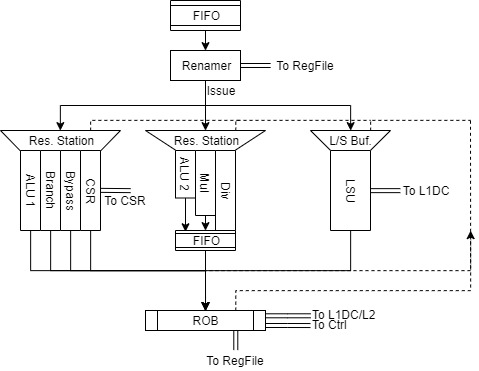
\includegraphics[width=0.8\textwidth]{assets/exec.jpg}
    \end{center}
  \end{columns}
\end{frame}

\begin{frame}
  \frametitle{Cache}
  \begin{columns}
    \column{0.3\textwidth}
    \begin{itemize}
      \item L1DC 分离 R/W
      \only<1>{
        \begin{itemize}
          \item R: sync, 1 cycle delay
          \item W: async
        \end{itemize}
      }
      \item MSI Directory
      \only<1>{
        \begin{itemize}
          \item 集中包含于 L2(LLC)
          \item 不包含 E 状态
        \end{itemize}
      }
      \item L2 兼当 AXI Crossbar
      \only<1>{
        \begin{itemize}
          \item<1> R Interleaving
        \end{itemize}
      }
      \only<2>{
        \item 可能发生 Reorder:
          \begin{itemize}
            \item WAW (WM)
            \item RAW
          \end{itemize}
        \item Atomic primitives
        \item TODO: mshr?
      }
    \end{itemize}
    \column{0.7\textwidth}
    \begin{center}
      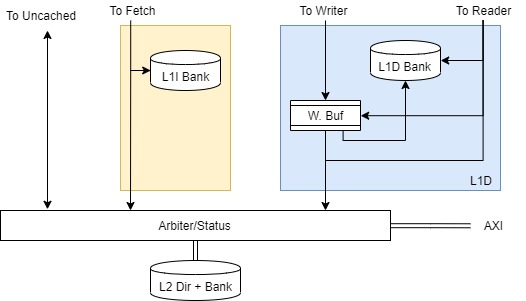
\includegraphics[width=0.8\textwidth]{assets/cache.jpg}
    \end{center}
  \end{columns}
\end{frame}

\begin{frame}
  \frametitle{Elaboration}
  \begin{columns}
    \column{0.3\textwidth}
    \begin{itemize}
      \item 7K LOC
      \item 70M
      \item About 50K LUT
    \end{itemize}
    \column{0.7\textwidth}
    \begin{center}
      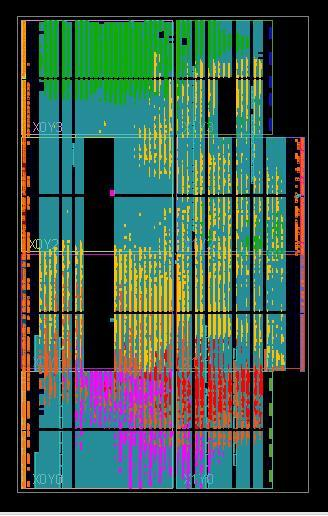
\includegraphics[width=0.5\textwidth]{assets/board.jpg}
    \end{center}
  \end{columns}
\end{frame}

\begin{frame}
  \frametitle{Chisel}
  \begin{columns}
    \column{0.3\textwidth}
    \begin{itemize}
      \item 可配置性非常强
      \item 保证线不会接错,但是存在部分隐式转换
      \item ILA 非常痛苦
    \end{itemize}
    \column{0.7\textwidth}
    \begin{center}
      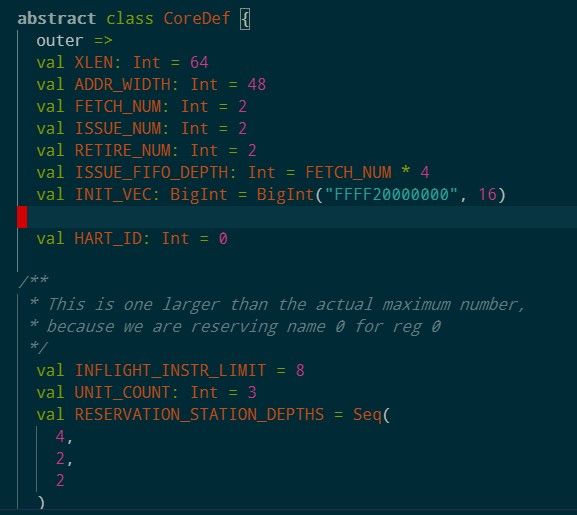
\includegraphics[width=\textwidth]{assets/def.jpg}
    \end{center}
  \end{columns}
\end{frame}

\begin{frame}
  \frametitle{Thanks!}
\end{frame}
\end{document}
